\documentclass[a4page]{article}

\usepackage{graphicx}
\usepackage{textpos}
\usepackage{hyperref}
\usepackage{xcolor}
\usepackage{enumitem}

\setitemize[1]{leftmargin=0ex,labelsep=10pt}

\newcommand\hsep{ {\color{gray}/} }
\newcommand\partitle[1]{\vskip20pt\par\noindent{\textsf{\textbf{#1}}}}

\usepackage{fontawesome}

\begin{document}

\begin{textblock}{2}(7,-.7)
    \noindent
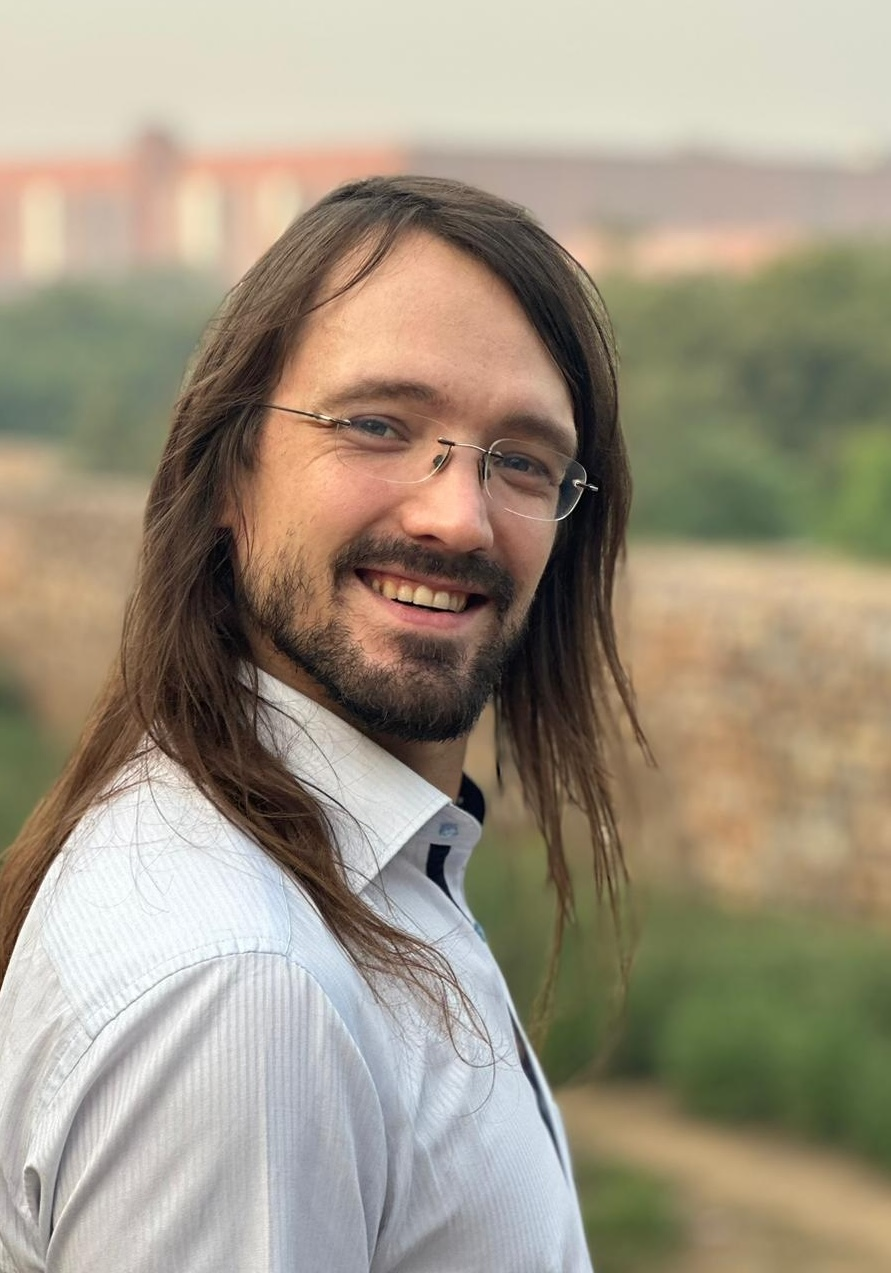
\includegraphics[width=\textwidth]{me2}
        \footnotesize(2023)
\end{textblock}\noindent
\textsf{\Large dr.~Bas Westerbaan}\\
curriculum vitae March~2025\\

\noindent
\href{mailto:bas@westerbaan.name}{\faEnvelopeO\ bas@westerbaan.name} \hsep
\href{https://bas.westerbaan.name}{\faExternalLink\ bas.westerbaan.name}\\
\href{https://scholar.google.nl/citations?user=AN7BEa8AAAAJ}{%
    \faGraduationCap\ Google Scholar}
    \hsep \href{https://github.com/bwesterb}{\faGithub\ \texttt{bwesterb}}
    \hsep \href{https://www.linkedin.com/in/baswesterbaan/}{\faLinkedinSquare} \\
$*$ 1988, the Netherlands

\vskip0.3cm\noindent

\partitle{Career}
\begin{itemize}
    \item[aug.~2021 -- present] \emph{Research engineer} --- Cloudflare\\
    I am the technical lead on Cloudflare's efforts to move
            the company itself and the Internet at large
            to post-quantum cryptography.
    My work ranges from implementation and
            measurement, to standardization and outreach.
    With the transition to post-quantum key agreement
        in the final phases,
            my current focus is preparing the WebPKI
    for \href{https://www.ietf.org/archive/id/draft-davidben-tls-merkle-tree-certs-00.html}{post-quantum certificates}.

        
    \item[2021] \emph{Cryptography engineer} --- PQShield\\
        I worked in the intersection of cryptography engineering and research,
            to mitigate some challenging cases.

    \item[2020] \emph{Post-doctoral researcher} (crypto engineering) --- Radboud Universiteit\\
        At the Digital Security group under prof.~Schwabe,
            I continued thinking about the practical challenges
                moving the Internet to post-quantum cryptography.
    \item[sept.~2020] \emph{Freelance developer} --- Stichting Privacy by Design\\
        I helped design, implement and deploy \href{https://qrona.info}{qrona.info}.
    \item[2019 -- 2020] \emph{Cryptography research fellow} (0.2fte) --- 
        \href{https://cloudflare.com}{Cloudflare} \\
        At the cryptography group of Nick Sullivan, I started my work
            on making the Internet secure against quantum computers.
        Already at this early fellowship,
            I embraced the breadth of the task:
            implementing various cryptographic primitives;
                performing large-scale experiments;
                designing changes to core protocols;
                and preparing internal infrastructure.

    \item[2019 -- 2020] \emph{Post-doctoral researcher} (1fte) --- University
        College London\\
        At the \href{http://pplv.cs.ucl.ac.uk/welcome/}{PPLV group}
            under \href{https://alexandrasilva.org/#/main.html}{prof.~dr.~Silva}.
    \item[2018 -- 2019] \emph{Cryptography engineer} --- Radboud Universiteit\\
        On the \href{https://pep.cs.ru.nl}{Polymorphic Encryption and Pseudonymisation (PEP) project}.
        Working with five colleagues, I made leaps in the practical usability
        of this data store at scale.

            
    \item[2013 -- 2018]  \emph{Promovendus (Ph.D-student) ---
        Radboud Universiteit}\\
        At the \href{http://www.ru.nl/ds/}{Digital Security group}
        of Radboud University funded by
        the ERC Advanced Grant \href{https://cordis.europa.eu/project/rcn/107285_en.html}{`Quantum Logic, Computation and Security'}
        of \href{http://www.cs.ru.nl/B.Jacobs/}{prof.~dr.~Bart Jacobs}.
            Defended
            \href{http://westerbaan.name/~bas/thesis.pdf}{thesis}
            on May 14th, 2019.
    \item[2007 -- 2013] \emph{B.Sc \& M.Sc degrees in Mathematics ---
                Radboud Universiteit} \\
        M.Sc thesis \href{www.ru.nl/publish/pages/813276/masterscriptie_bas_westerbaan.pdf}{`Sequential Product on Effect Logics'}
            supervised by \href{http://www.cs.ru.nl/B.Jacobs/}{prof.~dr.~Jacobs} \hsep
        B.Sc thesis \href{https://arxiv.org/abs/1409.1030}{`On Effective Undecidability and Post's Problem'}
            supervised by \href{http://www.ru.nl/wiskunde/@1039532/veldman-dhr-dr-(wim)/}{dr.~Veldman}.
        The Master's degree was awarded \emph{cum laude}.
    \item[2006 -- 2007] \emph{Freelance developer} (part-time)
        for software licensing database used by Dutch police.
\end{itemize}

\end{document}

% vim: ft=tex.latex
